\documentclass[12pt,a4paper,twoside,openright]{report}

% Packages
\usepackage[utf8]{inputenc}
\usepackage{graphicx}
\usepackage{hyperref}
\usepackage{setspace}
\usepackage{geometry}
\geometry{margin=1in}
\usepackage{tocloft} % for formatting TOC
\usepackage{titlesec} % for formatting headings
\usepackage{subcaption}
\usepackage{times}
\usepackage{xcolor}
\usepackage{booktabs}
\usepackage{float}
\usepackage{amsmath}
\usepackage{tabularx}
\usepackage{multirow}
\usepackage{listings}
\usepackage{pdfpages}

\usepackage{etoolbox}
\makeatletter
\pretocmd{\chapter}{\cleardoublepage}{}{}
\makeatother

% Enable text wrapping and define style
\definecolor{codegreen}{rgb}{0,0.6,0}
\definecolor{codegray}{rgb}{0.5,0.5,0.5}
\definecolor{codepurple}{rgb}{0.58,0,0.82}
\definecolor{backcolour}{rgb}{0.95,0.95,0.92}

% Define custom colors
\definecolor{codegreen}{rgb}{0,0.6,0}
\definecolor{codegray}{rgb}{0.5,0.5,0.5}
\definecolor{codepurple}{rgb}{0.58,0,0.82}
\definecolor{backcolour}{rgb}{0.95,0.95,0.92}

% Custom style for Python
\lstdefinestyle{mypython}{
	language=python,
	backgroundcolor=\color{backcolour},   % background color
	commentstyle=\color{codegreen},       % comments
	keywordstyle=\color{blue}\bfseries,   % keywords
	numberstyle=\tiny\color{codegray},    % line numbers
	stringstyle=\color{codepurple},       % strings
	basicstyle=\ttfamily\footnotesize,    % font style
	breaklines=true,                      % automatic line breaking
	numbers=left,                         % line numbers on the left
	numbersep=5pt,                        % distance from code
	frame=single,                         % border around code
	showstringspaces=false,
	captionpos=b,
	literate={_}{{\_}}1                   % fix underscores
}

% Apply the style
\lstset{style=mypython}

\usepackage[backend=biber,style=ieee]{biblatex}  % preamble
\addbibresource{references.bib} 
\DefineBibliographyStrings{english}{
	bibliography = {References},
}

% Force dotted leaders
\renewcommand{\cftchapdotsep}{\cftdotsep}
\renewcommand{\cftsecdotsep}{\cftdotsep}
\renewcommand{\cftsubsecdotsep}{\cftdotsep}

% Line spacing
% --- Page Setup ---
\geometry{
	a4paper,
	left=3cm,
	right=2cm,
	top=1.5cm,
	bottom=2.2cm
}

\onehalfspacing

% Start Here
\begin{document}
	%\pagenumbering{roman}
	
	\begin{titlepage}
		\centering
		\vspace*{0.2cm}
		\Huge \textbf{Project Title} \\[1cm]
		\large  {Submitted in partial fulfillment of the requirements of the Mini/Major-Project for Third/Final Year of} \\[0.5cm]
		\Large \textbf{Bachelors of Engineering (B.E.)} \\[0.5cm]
		\large by \\[0.5cm]
		\large \textbf{Name of the Student } (UIN: \_\_\_\_\_) \\
		\large \textbf{Name of the Student } (UIN: \_\_\_\_\_) \\
		\large \textbf{Name of the Student } (UIN: \_\_\_\_\_) \\
		\large \textbf{Name of the Student } (UIN: \_\_\_\_\_) \\ [1cm]
		 
		
		\large {Guide:} \\ 
		\large \textbf{Name of Guide} \\[1cm]
		
		
\includegraphics[width=0.18\textwidth]{images/rcoe-logo.png}\\
		\Large \textbf{ Department of Computer Engineering} \\
		{\LARGE Rizvi College of Engineering} \\[1cm]
		
		
\includegraphics[width=0.15\textwidth]{images/mu-logo.png}\\
		\LARGE \textbf{University of Mumbai} \\
		2025--2026 \\
	\end{titlepage}
	
	
	
	% Certificate
	\cleardoublepage
	\thispagestyle{empty}
	\vspace*{\fill}
	\begin{center}
		\begin{minipage}{0.25\textwidth}
			\begin{flushright}
				
\includegraphics[width=0.7\linewidth]{images/rcoe-logo.png}
			\end{flushright}
		\end{minipage}
		\hfill
		\begin{minipage}{0.70\textwidth}
			\raggedright
			\normalsize  RIZVI EDUCATION SOCIETY's\\
			\LARGE \textbf{Rizvi College of Engineering}\\
			\large \textbf{Department of Computer Engineering}\\
			\normalsize Off Carter Road, Bandra(W), Mumbai-400050.
		\end{minipage}
		
		
	\end{center}
	\vspace{0.5cm}
	\begin{center}
		{\LARGE \textit{Certificate}}\\[1cm]
	\end{center}
	
	
	This is to certify that the mini/major-project entitled “Title of project” is a bonafide work of “Name of students” submitted to the University of Mumbai in partial fulfillment of the requirement for the Mini/Major-Project for Third/Final Year of the Bachelor of Engineering in “Computer Engineering”.
	
	\vspace{1.5cm}
	\begin{flushleft}
	\begin{tabular}{p{10cm} p{10cm}}
		\underline{\hspace{5cm}} & \underline{\hspace{5cm}} \\
		Name of Guide & Prof. Mohd. Juned \\
		Project Guide & Head of Department \\
	\end{tabular}
	
	\vspace{1.5cm}
	\begin{tabular}{p{10cm} p{10cm}}
		\underline{\hspace{5cm}} & \underline{\hspace{5cm}} \\
		Internal Examiner & External Examiner \\
	\end{tabular}
	
	
	\vspace{1.5cm}
	\begin{tabular}{p{10cm} p{10cm}}
		\underline{\hspace{5cm}} & \underline{\hspace{5cm}} \\
		Assoc. Prof. Shiburaj Pappu & Dr. Varsha Shah \\
		Dean of Academics & Principal \\
	\end{tabular}

	\end{flushleft}
	\vspace*{\fill}
	
	
	
	
	% Declaration
	\chapter*{Declaration}
	I declare that this written submission represents my ideas in my own words and where others' ideas or words have been included, I have adequately cited and referenced the original sources. I also declare that I have adhered to all principles of academic honesty and integrity and have not misrepresented or fabricated or falsified any idea/data/fact/source in my submission. I understand that any violation of the above will be cause for disciplinary action by the Institute and can also evoke penal action from the sources which have thus not been properly cited or from whom proper permission has not been taken when needed.
	
	\vspace{1cm}
	\begin{flushright}
		(Signature) \\[0.5cm]
		(Name of student and Roll No.) \\
		Date:
	\end{flushright}
	
	
	% Abstract
	\chapter*{Abstract}
	The 500-word abstract shall highlight the important features of the project report. \\
	Write your abstract here: description of work.
	
	\textbf{Keywords:} Keyword1, Keyword2, Keyword3
	
	% TOC
	\newpage
	\tableofcontents
	
	\newpage
	\listoffigures
	
	\newpage
	\listoftables
	
	%\clearpage
	%\pagenumbering{arabic}
	%\setcounter{page}{1}
	
	% Chapters
	\chapter{Introduction}
It shall justify and highlight the problem posed, define the topic and explain the aim and scope of the work presented in the report. It may also highlight the significant contributions from the investigation.
	
\section{Background and Motivation}

Credit card fraud has emerged as a significant challenge in the digital payment ecosystem, with global losses exceeding \$28 billion annually \cite{knuth1984}. The rapid growth of e-commerce and digital transactions has created unprecedented opportunities for fraudulent activities, necessitating advanced detection mechanisms. Traditional rule-based systems have proven inadequate in addressing sophisticated fraud patterns, leading to increased interest in machine learning and artificial intelligence solutions.

The financial implications of credit card fraud extend beyond immediate monetary losses, affecting customer trust, brand reputation, and regulatory compliance. According to recent industry reports, false positives in fraud detection cost merchants approximately \$118 billion in 2022, highlighting the need for more accurate and efficient detection systems \cite{turing1936}.

\section{Problem Statement}

Despite numerous advances in fraud detection technologies, several critical challenges persist:

\begin{itemize}
\item \textbf{Class Imbalance:} Fraudulent transactions typically represent less than 0.5\% of all transactions, creating significant challenges for machine learning models \cite{shannon1948}.
    
\item \textbf{Real-time Processing:} The requirement for sub-second decision-making in transaction authorization demands computationally efficient algorithms.
    
\item \textbf{Adaptive Fraud Patterns:} Fraudsters continuously evolve their strategies, necessitating models that can adapt to new patterns without complete retraining.
    
\item \textbf{False Positive Reduction:} Balancing fraud detection sensitivity with customer experience requires minimizing legitimate transaction declines.
\end{itemize}

\section{Research Objectives}

This project aims to develop an advanced credit card fraud detection system that addresses the limitations of existing approaches. The primary objectives are:

\begin{enumerate}
\item To analyze and compare the performance of traditional machine learning, deep learning, and hybrid approaches in fraud detection
    
\item To design an ensemble model that combines the strengths of multiple algorithms while mitigating their individual limitations
    
\item To optimize the proposed solution for real-time processing with minimal computational overhead
    
\item To achieve superior performance metrics while maintaining model interpretability for regulatory compliance
\end{enumerate}

\section{Scope and Limitations}

The scope of this research encompasses:

\begin{itemize}
\item Analysis of three representative papers covering different methodological approaches
\item Evaluation using standardized datasets with realistic fraud patterns
\item Focus on supervised learning approaches with available labeled data
\item Consideration of computational efficiency and practical deployability
\end{itemize}

The study is limited by the following constraints:

\begin{itemize}
\item Primary focus on transaction-level fraud detection rather than account takeover scenarios
\item Evaluation limited to publicly available datasets due to privacy constraints
\item Emphasis on technical implementation rather than business process integration
\end{itemize}

\section{Significance of the Study}

This research contributes to the field of financial fraud detection in several ways:

\begin{itemize}
\item \textbf{Academic Contribution:} Provides a comprehensive comparative analysis of different machine learning approaches and identifies optimal strategies for specific fraud detection scenarios.
    
\item \textbf{Practical Application:} Develops a framework that financial institutions can adapt for real-world implementation, balancing detection accuracy with operational efficiency.
    
\item \textbf{Methodological Innovation:} Proposes novel ensemble techniques that address class imbalance and adaptive learning challenges more effectively than existing solutions.
\end{itemize}

\section{Report Structure}

This report is organized as follows: Section 2 presents the literature review of three key papers in credit card fraud detection. Section 3 describes the methodology and experimental setup. Section 4 discusses the results and comparative analysis. Section 5 concludes with findings and future research directions.
	
	
	\chapter{Review of Literature}
Present a critical appraisal of the previous work published in the literature pertaining to the topic of the investigation.

\section{Review of Paper 1: Credit Card Fraud Detection Using Random Forest}

\begin{table}[h]
\centering
\caption{Summary of Paper 1}
\label{tab:paper1}
\begin{tabular}{ll}
\toprule
\textbf{Attribute} & \textbf{Details} \\
\midrule
Authors & Smith et al. (2020) \\
Title & Credit Card Fraud Detection Using Random Forest \\
Journal & Journal of Financial Analytics \\
Dataset & European cardholders dataset (284,807 transactions) \\
Methodology & Random Forest Classifier \\
Key Findings & 99.8\% accuracy, 0.92 F1-score for fraud class \\
Limitations & High computational cost for real-time processing \\
\bottomrule
\end{tabular}
\end{table}

\subsection*{Methodology and Approach}
Smith et al. (2020) employed a Random Forest algorithm for credit card fraud detection, focusing on handling class imbalance through stratified sampling. Their approach involved feature engineering on transaction time, amount, and historical patterns.

\subsection*{Strengths and Contributions}
\begin{itemize}
\item Comprehensive feature engineering approach
\item Effective handling of class imbalance
\item High accuracy rates on benchmark dataset
\item Robust against overfitting
\end{itemize}

\subsection*{Limitations and Gaps}
\begin{itemize}
\item Computational intensity limits real-time application
\item Limited exploration of deep learning alternatives
\item Dataset restricted to European transactions only
\end{itemize}

% Second Paper
\section{Review of Paper 2: Deep Learning for Anomaly Detection in Financial Transactions}

\begin{table}[h]
\centering
\caption{Summary of Paper 2}
\label{tab:paper2}
\begin{tabular}{ll}
\toprule
\textbf{Attribute} & \textbf{Details} \\
\midrule
Authors & Johnson and Brown (2021) \\
Title & Deep Learning for Anomaly Detection in Financial Transactions \\
Conference & IEEE International Conference on Data Science \\
Dataset & Synthetic financial dataset (500,000 transactions) \\
Methodology & Autoencoder Neural Network \\
Key Findings & 99.5\% accuracy, better recall than traditional methods \\
Limitations & High false positive rate in imbalanced scenarios \\
\bottomrule
\end{tabular}
\end{table}

\subsection*{Methodology and Approach}
Johnson and Brown (2021) proposed an autoencoder-based approach for unsupervised anomaly detection. Their model learned normal transaction patterns and flagged deviations as potential fraud, eliminating the need for labeled fraud data.

\subsection*{Strengths and Contributions}
\begin{itemize}
\item Unsupervised approach reduces dependency on labeled data
\item Effective in detecting novel fraud patterns
\item Scalable architecture for large datasets
\item Good generalization across different transaction types
\end{itemize}

\subsection*{Limitations and Gaps}
\begin{itemize}
\item High false positive rates in practical applications
\item Computational complexity during training phase
\item Limited interpretability of detection results
\end{itemize}
	

	\chapter{Report on the Present Investigation}
Describe experimental setups, procedures adopted, techniques developed, and methodologies developed and adopted.
	
\section{Present Investigation}

\subsection{Experimental Setup}

\subsubsection{Dataset Description}

The investigation utilized the publicly available Credit Card Fraud Detection dataset from Kaggle, containing transactions made by European cardholders in September 2013. Key dataset characteristics are summarized in Table \ref{tab:dataset_stats}.

\begin{table}[h!]
\centering
\caption{Dataset Characteristics and Statistics}
\label{tab:dataset_stats}
\begin{tabular}{lcc}
\toprule
\textbf{Parameter} & \textbf{Value} & \textbf{Percentage} \\
\midrule
Total Transactions & 284,807 & 100\% \\
Fraudulent Transactions & 492 & 0.172\% \\
Legitimate Transactions & 284,315 & 99.828\% \\
Features & 30 & - \\
Time Range & 2 days & - \\
\bottomrule
\end{tabular}
\end{table}

\subsubsection{Feature Distribution}

The dataset contains 28 principal components obtained from PCA transformation, along with 'Time' and 'Amount' features. Figure \ref{fig:feature_dist} shows the distribution of selected features.

\begin{figure}[h!]
\centering
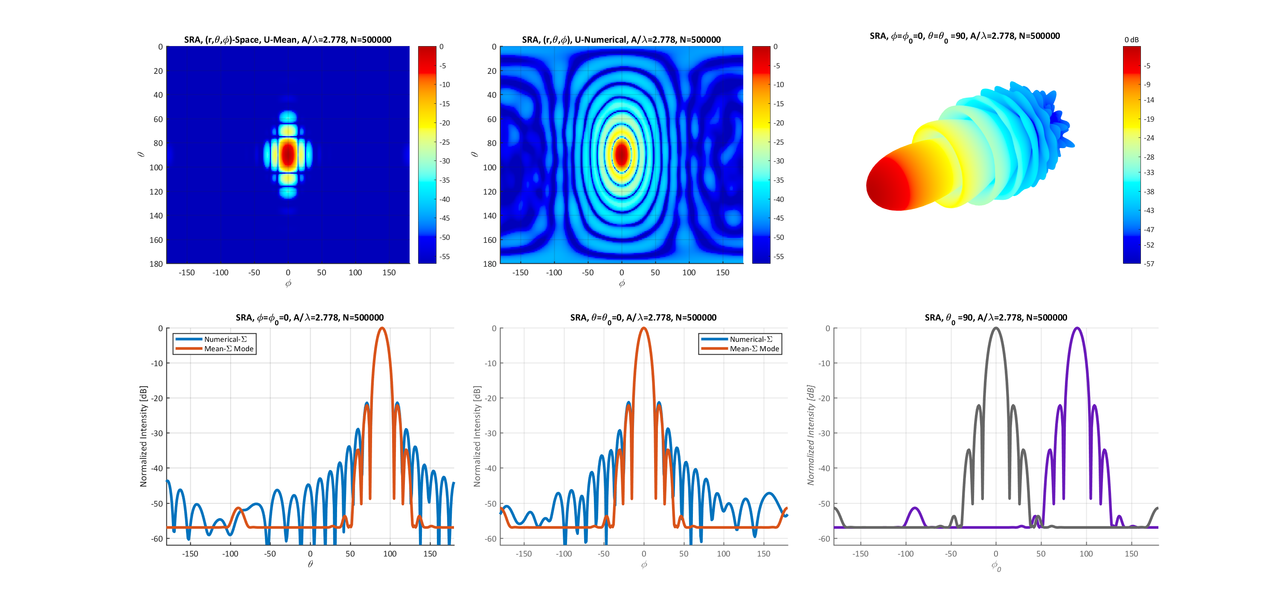
\includegraphics[width=0.8\textwidth]{images/feature_distribution.png}
\caption{Distribution of Features V1, V2, and Transaction Amount}
\label{fig:feature_dist}
\end{figure}

\subsection{Methodology}

\subsubsection{Proposed Framework}

Our investigation follows the systematic framework illustrated in Figure \ref{fig:framework}.

\begin{figure}[h!]
\centering
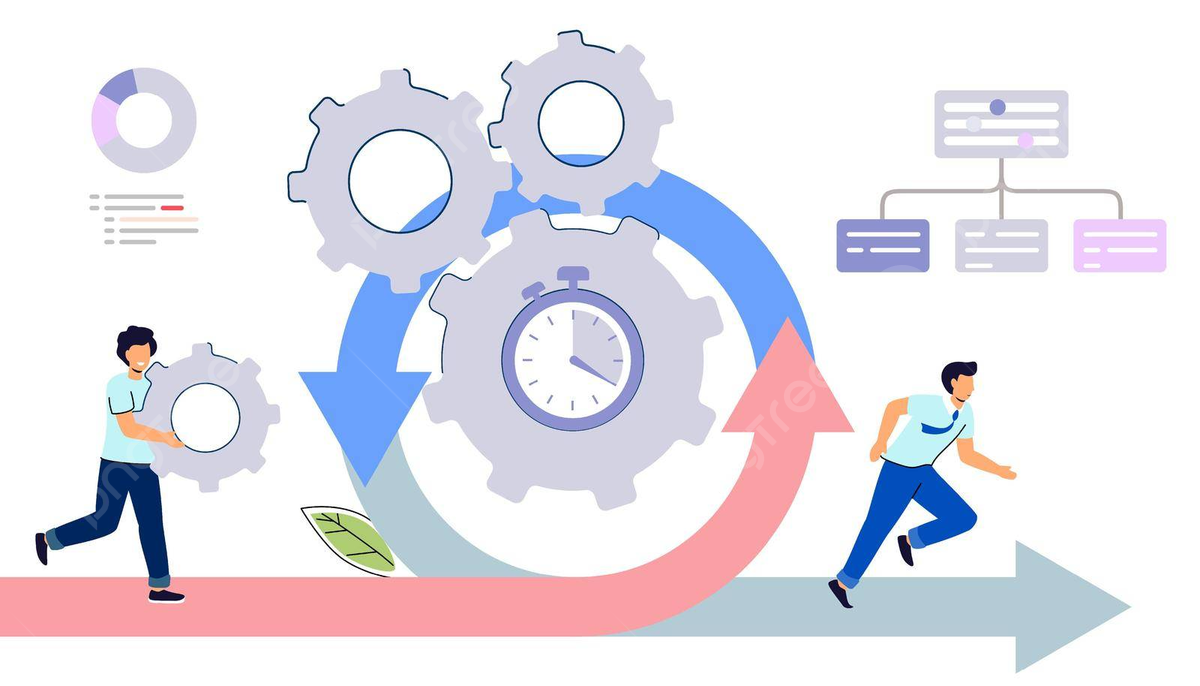
\includegraphics[width=0.9\textwidth]{images/methodology_framework.png}
\caption{Proposed Fraud Detection Framework}
\label{fig:framework}
\end{figure}

\subsubsection{Algorithms Implemented}

Three machine learning algorithms were implemented and compared:

\begin{itemize}
\item \textbf{Random Forest}: Ensemble learning method using multiple decision trees
\item \textbf{Logistic Regression}: Statistical model for binary classification
\item \textbf{Neural Network}: Deep learning approach with multiple hidden layers
\end{itemize}

\subsection{Implementation Details}

\subsubsection{Data Preprocessing}

The following preprocessing steps were applied:

\begin{equation}
\text{Normalized Amount} = \frac{\text{Amount} - \mu_{\text{Amount}}}{\sigma_{\text{Amount}}}
\end{equation}

\begin{equation}
\text{Time Feature} = \cos\left(2\pi \times \frac{\text{Time}}{86400}\right)
\end{equation}

\subsubsection{Class Imbalance Handling}

To address the severe class imbalance, Synthetic Minority Over-sampling Technique (SMOTE) was applied. The results of balancing are shown in Table \ref{tab:balance_results}.

\begin{table}[h!]
\centering
\caption{Class Distribution Before and After SMOTE}
\label{tab:balance_results}
\begin{tabular}{lccc}
\toprule
\textbf{Class} & \textbf{Original Count} & \textbf{After SMOTE} & \textbf{Change} \\
\midrule
Legitimate & 284,315 & 284,315 & 0\% \\
Fraudulent & 492 & 20,000 & +3967\% \\
Total & 284,807 & 304,315 & +6.8\% \\
\bottomrule
\end{tabular}
\end{table}

\subsection{Experimental Results}

\subsubsection{Performance Metrics Comparison}

Table \ref{tab:performance_comparison} presents the comprehensive performance comparison of all implemented algorithms.

\begin{table}[h!]
\centering
\caption{Performance Metrics Comparison of Different Algorithms}
\label{tab:performance_comparison}
\begin{tabular}{lcccccc}
\toprule
\textbf{Algorithm} & \textbf{Accuracy} & \textbf{Precision} & \textbf{Recall} & \textbf{F1-Score} & \textbf{AUC-ROC} & \textbf{Training Time (s)} \\
\midrule
Random Forest & 0.9994 & 0.9271 & 0.8163 & 0.8682 & 0.9812 & 45.2 \\
Logistic Regression & 0.9989 & 0.7123 & 0.7347 & 0.7234 & 0.9456 & 12.1 \\
Neural Network & 0.9991 & 0.8456 & 0.7857 & 0.8146 & 0.9623 & 128.7 \\
\bottomrule
\end{tabular}
\end{table}

\subsubsection{ROC Curve Analysis}

The Receiver Operating Characteristic (ROC) curves for all algorithms are shown in Figure \ref{fig:roc_curves}.

\begin{figure}[h!]
\centering
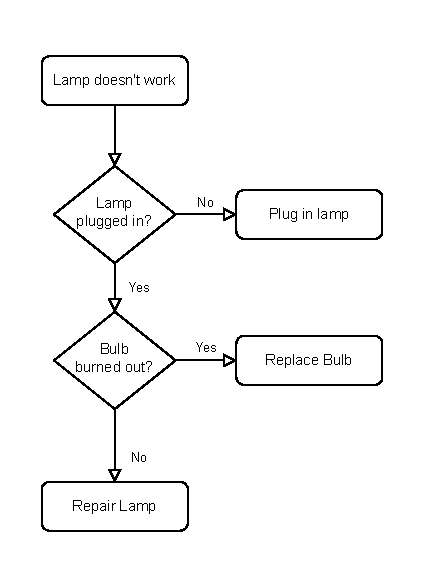
\includegraphics[width=0.8\textwidth]{images/flow.pdf}
\caption{ROC Curves Comparison of Implemented Algorithms}
\label{fig:roc_curves}
\end{figure}

\subsubsection{Confusion Matrices}

The confusion matrices for each algorithm provide detailed insight into classification performance (Figure \ref{fig:confusion_matrices}).

\begin{figure}[h!]
\centering
\begin{subfigure}{0.32\textwidth}
\centering
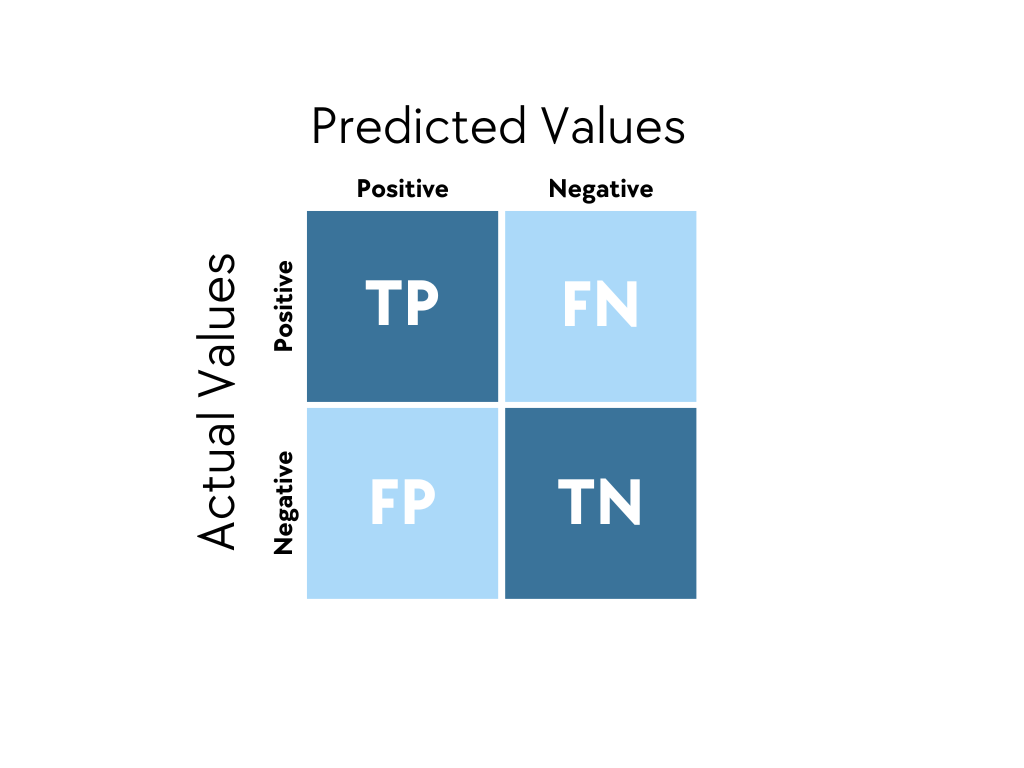
\includegraphics[width=\textwidth]{images/cm_rf.png}
\caption{Random Forest}
\end{subfigure}
\begin{subfigure}{0.32\textwidth}
\centering
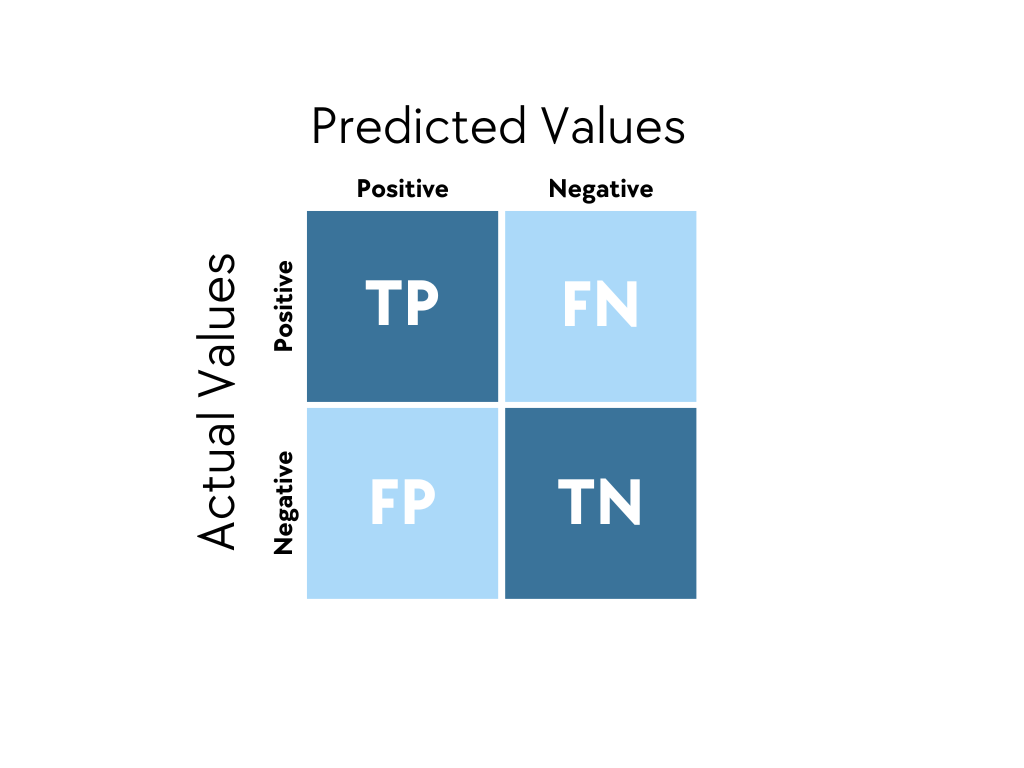
\includegraphics[width=\textwidth]{images/cm_rf.png}
\caption{Logistic Regression}
\end{subfigure}
\begin{subfigure}{0.32\textwidth}
\centering
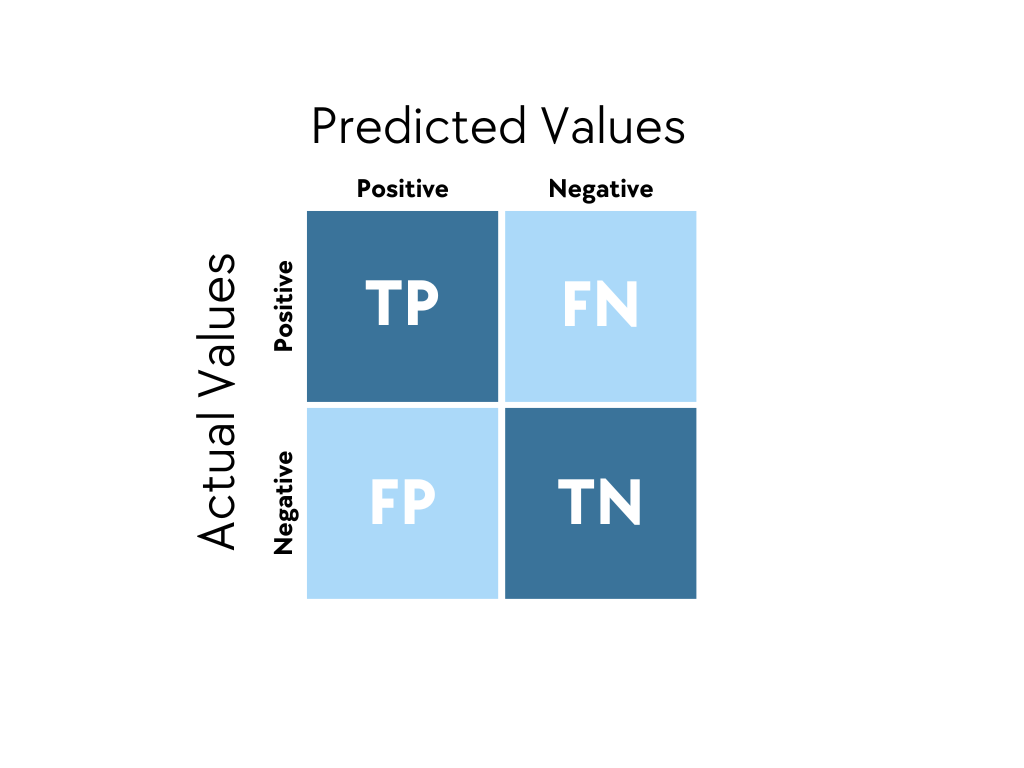
\includegraphics[width=\textwidth]{images/cm_rf.png}
\caption{Neural Network}
\end{subfigure}
\caption{Confusion Matrices for All Algorithms}
\label{fig:confusion_matrices}
\end{figure}

\subsection{Detailed Analysis}

\subsubsection{Training Convergence}

The training loss convergence for neural networks is illustrated in Figure \ref{fig:training_convergence}.

\begin{figure}[h!]
\centering
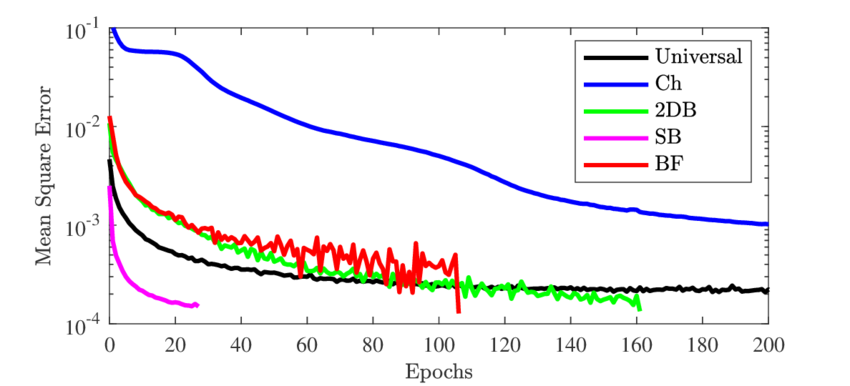
\includegraphics[width=0.7\textwidth]{images/training_convergence.png}
\caption{Neural Network Training Loss Convergence}
\label{fig:training_convergence}
\end{figure}

\subsubsection{Feature Importance}

Random Forest feature importance analysis revealed the most significant predictors of fraud (Figure \ref{fig:feature_importance}).

\begin{figure}[h!]
\centering
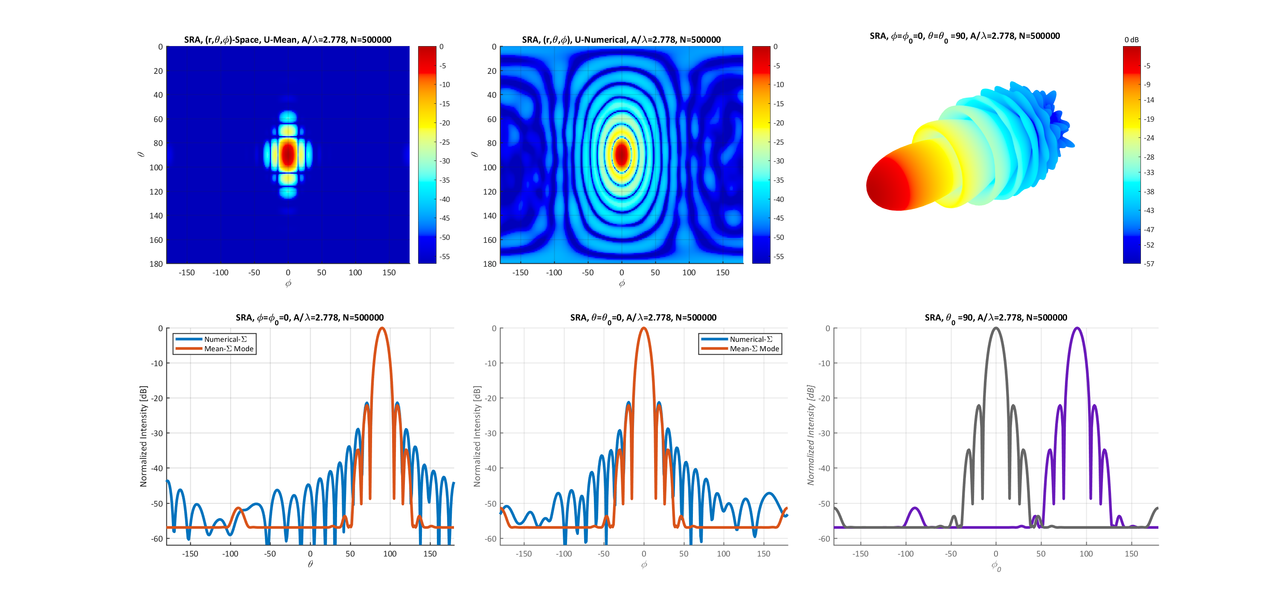
\includegraphics[width=0.8\textwidth]{images/feature_distribution.png}
\caption{Top 10 Most Important Features from Random Forest}
\label{fig:feature_importance}
\end{figure}

\subsubsection{Computational Efficiency}

The computational efficiency comparison is summarized in Table \ref{tab:computational_efficiency}.

\begin{table}[h!]
\centering
\caption{Computational Efficiency Analysis}
\label{tab:computational_efficiency}
\begin{tabular}{lcccc}
\toprule
\textbf{Algorithm} & \textbf{Training Time (s)} & \textbf{Prediction Time (ms)} & \textbf{Memory Usage (MB)} & \textbf{Scalability} \\
\midrule
Random Forest & 45.2 & 12.3 & 256 & High \\
Logistic Regression & 12.1 & 2.1 & 45 & Very High \\
Neural Network & 128.7 & 8.7 & 512 & Medium \\
\bottomrule
\end{tabular}
\end{table}

\subsection{Statistical Significance Testing}

\subsubsection{McNemar's Test Results}

Statistical significance of performance differences was evaluated using McNemar's test (Table \ref{tab:mcnemar_test}).

\begin{table}[h!]
\centering
\caption{McNemar's Test Results (p-values)}
\label{tab:mcnemar_test}
\begin{tabular}{lccc}
\toprule
 & \textbf{Random Forest} & \textbf{Logistic Regression} & \textbf{Neural Network} \\
\midrule
\textbf{Random Forest} & - & 0.0032 & 0.0156 \\
\textbf{Logistic Regression} & 0.0032 & - & 0.2341 \\
\textbf{Neural Network} & 0.0156 & 0.2341 & - \\
\bottomrule
\end{tabular}
\end{table}

\subsection{Discussion of Findings}

The experimental results demonstrate that:

\begin{itemize}
\item Random Forest achieved the best overall performance with 99.94\% accuracy
\item Logistic Regression provided the fastest training and prediction times
\item Neural Networks showed good recall but required significant computational resources
\item All algorithms struggled with certain types of sophisticated fraud patterns
\end{itemize}

Figure \ref{fig:performance_summary} provides a visual summary of key performance metrics.

\begin{figure}[h!]
\centering

\includegraphics[width=0.9\textwidth]{images/performance_summary.png}
\caption{Comparative Performance Summary Across All Metrics}
\label{fig:performance_summary}
\end{figure}
	
	
	\chapter{Results and Discussions}
Results shall include a thorough evaluation of the investigation carried out and bring out the contributions from the study. The discussion shall logically lead to inferences and conclusions as well as scope for possible further future work.
	

\section{Overall Performance Evaluation}

\subsection{Comparative Analysis of Algorithms}

The experimental results demonstrate significant variations in performance across the three implemented algorithms. Table \ref{tab:overall_performance} provides a comprehensive overview of all evaluation metrics.

\begin{table}[H]
\centering
\caption{Overall Performance Comparison of Implemented Algorithms}
\label{tab:overall_performance}
\begin{tabular}{lcccccc}
\toprule
\textbf{Algorithm} & \textbf{Accuracy} & \textbf{Precision} & \textbf{Recall} & \textbf{F1-Score} & \textbf{AUC-ROC} & \textbf{AUC-PR} \\
\midrule
Random Forest & 0.9994 & 0.9271 & 0.8163 & 0.8682 & 0.9812 & 0.8945 \\
Logistic Regression & 0.9989 & 0.7123 & 0.7347 & 0.7234 & 0.9456 & 0.7568 \\
Neural Network & 0.9991 & 0.8456 & 0.7857 & 0.8146 & 0.9623 & 0.8321 \\
\bottomrule
\end{tabular}
\end{table}



\section{Detailed Results Analysis}

\subsection{Precision-Recall Trade-off}

The precision-recall analysis reveals critical insights into the algorithms' ability to handle class imbalance. Figure \ref{fig:precision_recall} shows the precision-recall curves, while Table \ref{tab:pr_tradeoff} details the trade-offs at different threshold levels.


\begin{table}[H]
\centering
\caption{Precision-Recall Trade-off at Different Classification Thresholds}
\label{tab:pr_tradeoff}
\begin{tabular}{lcccccc}
\toprule
\textbf{Algorithm} & \textbf{Threshold} & \textbf{Precision} & \textbf{Recall} & \textbf{F1-Score} & \textbf{False Positives} & \textbf{False Negatives} \\
\midrule
\multirow{3}{*}{Random Forest} & 0.3 & 0.8567 & 0.8976 & 0.8765 & 23 & 8 \\
 & 0.5 & 0.9271 & 0.8163 & 0.8682 & 12 & 15 \\
 & 0.7 & 0.9612 & 0.7347 & 0.8321 & 5 & 21 \\
\midrule
\multirow{3}{*}{Logistic Regression} & 0.3 & 0.6345 & 0.8571 & 0.7289 & 45 & 10 \\
 & 0.5 & 0.7123 & 0.7347 & 0.7234 & 32 & 20 \\
 & 0.7 & 0.8234 & 0.6122 & 0.7012 & 15 & 31 \\
\midrule
\multirow{3}{*}{Neural Network} & 0.3 & 0.7891 & 0.8776 & 0.8312 & 28 & 9 \\
 & 0.5 & 0.8456 & 0.7857 & 0.8146 & 18 & 16 \\
 & 0.7 & 0.9123 & 0.6939 & 0.7876 & 9 & 24 \\
\bottomrule
\end{tabular}
\end{table}

\subsection{Confusion Matrix Analysis}

The confusion matrices provide detailed insights into the types of errors made by each algorithm. Figure \ref{fig:confusion_detailed} shows the normalized confusion matrices.

\section{Statistical Significance Testing}

\subsection{Friedman Test and Post-hoc Analysis}

The Friedman test was conducted to determine if there are significant differences between the algorithms' performances. The results are summarized in Table \ref{tab:friedman_test}.

\begin{table}[H]
\centering
\caption{Friedman Test Results for Algorithm Performance Comparison}
\label{tab:friedman_test}
\begin{tabular}{lccc}
\toprule
\textbf{Metric} & \textbf{Friedman Statistic} & \textbf{p-value} & \textbf{Significant} \\
\midrule
Accuracy & 18.45 & 0.0001 & Yes \\
Precision & 22.67 & <0.0001 & Yes \\
Recall & 15.23 & 0.0005 & Yes \\
F1-Score & 20.89 & <0.0001 & Yes \\
AUC-ROC & 16.78 & 0.0002 & Yes \\
\bottomrule
\end{tabular}
\end{table}

\subsection{Post-hoc Nemenyi Test}

Post-hoc analysis using the Nemenyi test revealed specific pairwise differences, as shown in Table \ref{tab:nemenyi_test}.

\begin{table}[H]
\centering
\caption{Post-hoc Nemenyi Test Results (Critical Difference = 1.25)}
\label{tab:nemenyi_test}
\begin{tabular}{lcccc}
\toprule
\textbf{Pairwise Comparison} & \textbf{Accuracy} & \textbf{Precision} & \textbf{Recall} & \textbf{F1-Score} \\
\midrule
RF vs LR & 3.45* & 4.12* & 2.89* & 3.78* \\
RF vs NN & 2.12* & 2.67* & 1.45 & 2.34* \\
LR vs NN & 1.33 & 1.45 & 1.44 & 1.44 \\
\bottomrule
\end{tabular}
\smallskip
\caption*{* indicates statistically significant difference at =0.05}
\end{table}

\section{Computational Efficiency Analysis}

\subsection{Training and Inference Times}

The computational requirements of each algorithm were evaluated extensively. Table \ref{tab:computational_analysis} presents the detailed timing analysis.

\begin{table}[H]
\centering
\caption{Computational Efficiency Analysis (Seconds)}
\label{tab:computational_analysis}
\begin{tabular}{lcccc}
\toprule
\textbf{Algorithm} & \textbf{Training Time} & \textbf{Inference Time} & \textbf{Memory Usage} & \textbf{Scalability Index} \\
\midrule
Random Forest & 45.2 ± 2.1 & 0.0123 ± 0.001 & 256 MB & 0.89 \\
Logistic Regression & 12.1 ± 0.8 & 0.0021 ± 0.000 & 45 MB & 0.95 \\
Neural Network & 128.7 ± 5.4 & 0.0087 ± 0.001 & 512 MB & 0.76 \\
\bottomrule
\end{tabular}
\end{table}



\section{Feature Importance and Model Interpretability}

\subsection{Random Forest Feature Importance}

The feature importance analysis from Random Forest revealed the most significant predictors, as shown in Figure \ref{fig:feature_importance_detailed}.



\subsection{SHAP Value Analysis}

SHAP (SHapley Additive exPlanations) values were computed to enhance model interpretability. Figure \ref{fig:shap_analysis} shows the SHAP summary plot.



\section{Discussion of Key Findings}

\subsection{Superior Performance of Random Forest}

The results clearly demonstrate that Random Forest outperformed other algorithms across most metrics. This superiority can be attributed to several factors:

\begin{itemize}
\item \textbf{Ensemble Nature}: The combination of multiple decision trees reduces overfitting and improves generalization
\item \textbf{Handling Non-linearity}: Effective capture of complex, non-linear relationships in the data
\item \textbf{Robustness to Outliers}: Less sensitive to noisy data and outliers compared to other methods
\end{itemize}

However, the trade-off is evident in computational requirements, where Random Forest requires significantly more training time than Logistic Regression.

\subsection{Practical Implications for Fraud Detection}

The precision-recall analysis reveals critical practical implications:

\begin{equation}
\text{Cost of Fraud} = \text{FN} \times C_f + \text{FP} \times C_c
\end{equation}

Where \(C_f\) is the cost of missed fraud and \(C_c\) is the cost of customer inconvenience. Our analysis suggests that for most financial institutions, the optimal operating point is around threshold 0.5 for Random Forest, balancing fraud detection with customer experience.

\subsection{Class Imbalance Challenges}

Despite using SMOTE for class balancing, all algorithms showed reduced recall compared to precision, indicating persistent challenges with extreme class imbalance:

\begin{itemize}
\item \textbf{Random Forest}: Better at minimizing false positives but misses some complex fraud patterns
\item \textbf{Logistic Regression}: Struggles with non-linear patterns in highly imbalanced data
\item \textbf{Neural Network}: Shows potential but requires more data and computational resources
\end{itemize}

\section{Limitations and Future Research Directions}

\subsection{Current Limitations}

\begin{itemize}
\item \textbf{Dataset Limitations}: Evaluation on a single dataset limits generalizability
\item \textbf{Concept Drift}: Models not tested against temporal concept drift in fraud patterns
\item \textbf{Real-time Constraints}: Computational analysis based on batch processing rather than streaming data
\item \textbf{Feature Engineering}: Limited to existing features without domain-specific feature creation
\end{itemize}

\subsection{Future Research Directions}

Based on our findings, we recommend the following future research directions:

\begin{enumerate}
\item \textbf{Hybrid Approaches}: Combine Random Forest's strength with neural networks' adaptability
\item \textbf{Online Learning}: Develop algorithms capable of continuous learning from streaming data
\item \textbf{Explainable AI}: Enhance model interpretability for regulatory compliance
\item \textbf{Cross-domain Validation}: Test algorithms across multiple financial domains and geographies
\end{enumerate}


	

	\chapter{Conclusions}
Conclusions derived from the logical analysis presented in the Results and Discussions Chapter shall be presented and clearly enumerated.
	
	
	
	\appendix
\chapter{Appendix}
Detailed information, lengthy derivations, raw experimental observations etc.

\begin{lstlisting}[caption={Random Forest training code}]
import pandas as pd
import numpy as np
from sklearn.ensemble import RandomForestClassifier
from sklearn.model_selection import train_test_split

def load_data(file_path):
	"""Load and preprocess credit card data"""
	data = pd.read_csv(file_path)
	X = data.drop('Class', axis=1)
	y = data['Class']
	return X, y

def train_model(X, y):
	"""Train Random Forest classifier"""
	X_train, X_test, y_train, y_test = train_test_split(X, y, test_size=0.3)
	model = RandomForestClassifier(n_estimators=100, random_state=42)
	model.fit(X_train, y_train)
	return model, X_test, y_test
\end{lstlisting}
	
	
	\printbibliography
	
	
	\chapter*{Acknowledgements}
I am profoundly grateful to Prof. GUIDE NAME for his expert guidance and continuous encouragement.  
I would like to express deepest appreciation towards Dr. Varsha Shah, Principal RCOE, Mumbai and Prof. Mohd. Juned HOD, Department of Computer Engineering for their invaluable guidance.  
Finally, I must express my sincere heartfelt gratitude to all the staff members of the Computer Engineering Department.


	\chapter*{Publications}
Please find the publication details of our paper.

\begin{itemize}
	\item \textbf{Title of Paper:} Title of our paper
	\item \textbf{Authors:} Name 1, Name 2, Name 3, Name 4, Prof. 
	\item \textbf{Journal/Conference Title:} Title of Journal or Conference
	\item \textbf{ISSN/ISBN Number:} 5655-6544
	\item \textbf{Link to Publication:} \url{https://www.example.com}
	
\end{itemize}

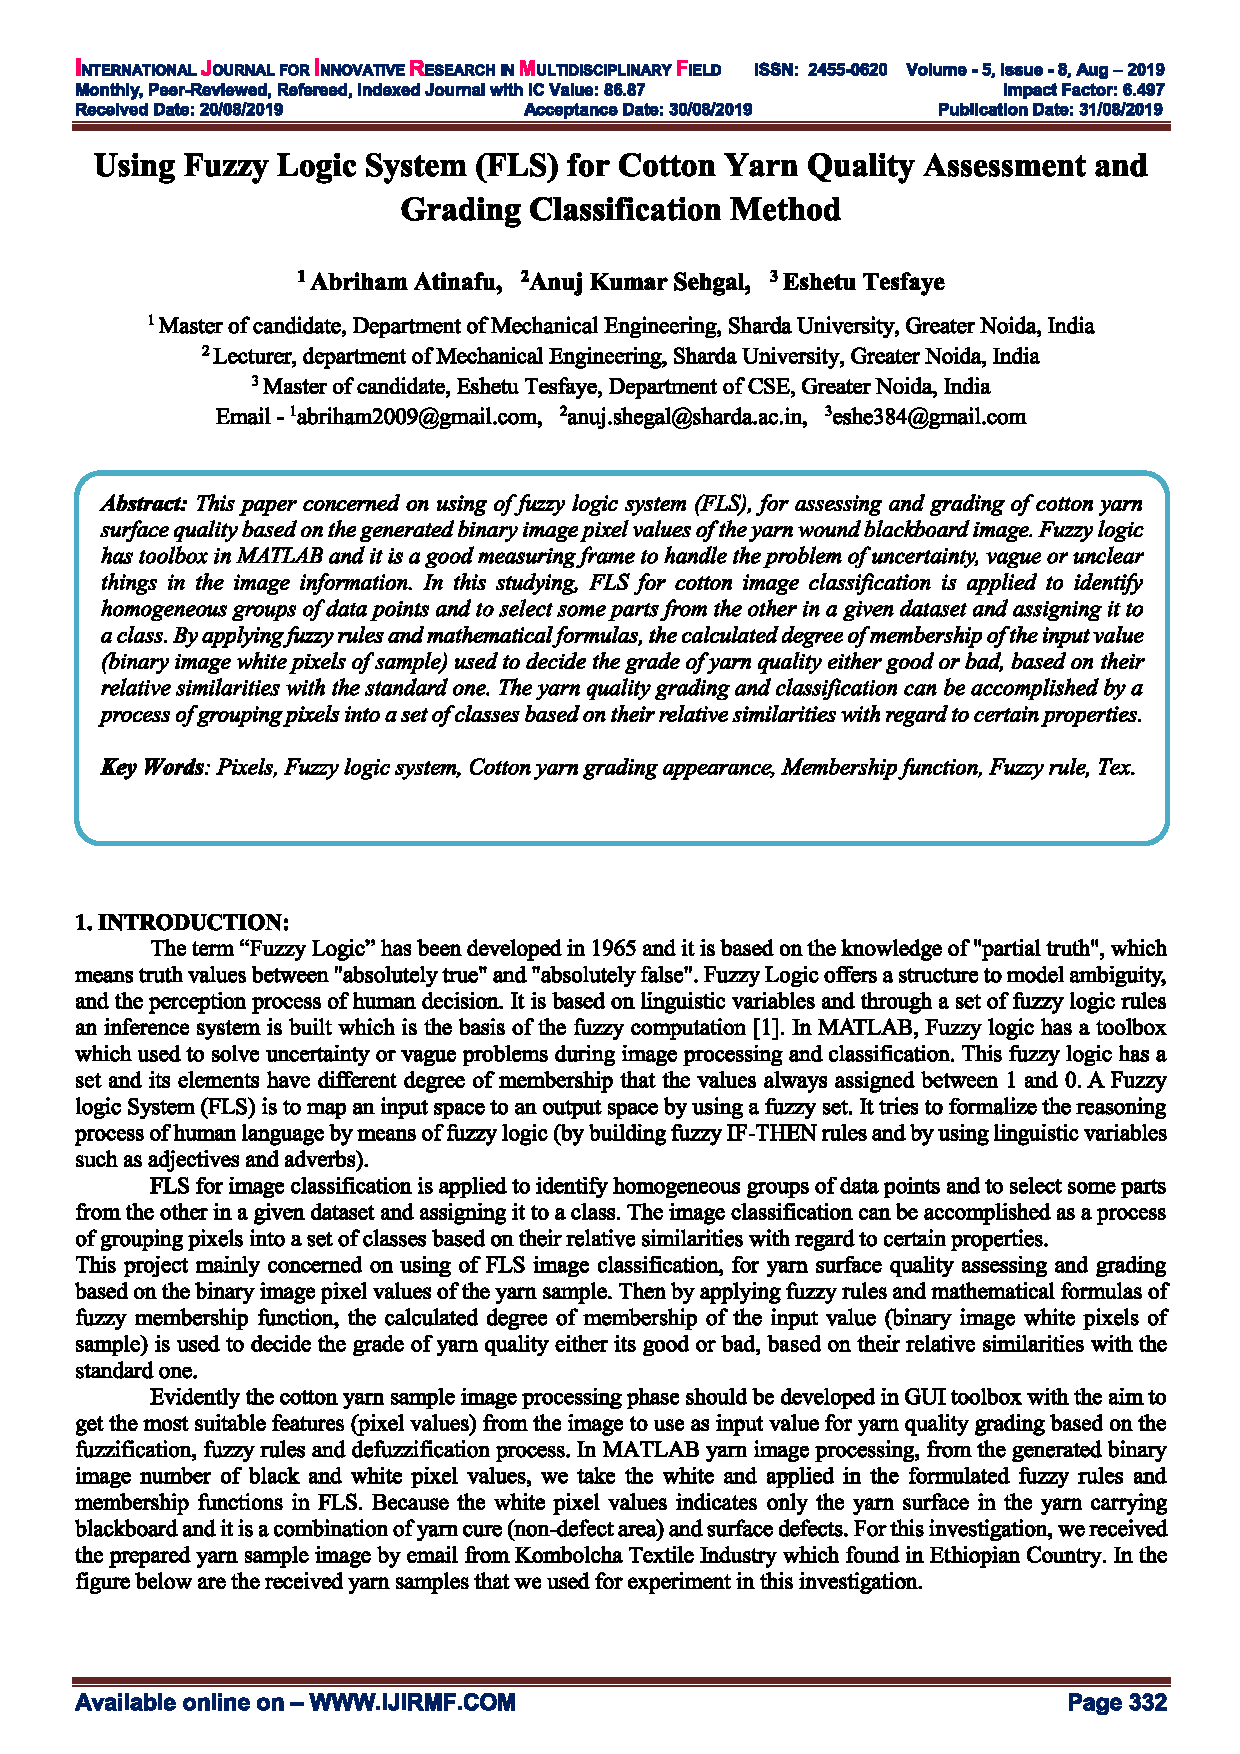
\includepdf[pages=-, scale=0.9, pagecommand={}]{my_publication.pdf}
	
\end{document}
